\documentclass[11pt]{article}
\usepackage[a4paper, margin=20mm]{geometry}
 

\usepackage{amsmath}
\usepackage{physics}

\usepackage{graphicx}
\graphicspath{ {./figs/} }
\usepackage{subfig}

%\renewcommand{\baselinestretch}{2}
\usepackage{setspace}
\doublespacing
\usepackage{titlesec}

\titlespacing\section{0pt}{0pt plus 0pt minus 0pt}{0pt plus 2pt minus 2pt}
\titlespacing\subsection{0pt}{0pt plus 4pt minus 2pt}{0pt plus 2pt minus 2pt}
\titlespacing\subsubsection{0pt}{0pt plus 4pt minus 2pt}{0pt plus 2pt minus 2pt}



\begin{document}

\section{Data Pre-processing}
The reading date and time were given in ISO format, so they were converted into seconds with the earliest datetime (2007-05-26T12:05:00) as the zero reference, i.e. the difference between a given datetime and the earliest datetime were calculated in terms of seconds. The 'Time (s)' values in the graphs reflect these calculations.

\section{Exponentiated Quadratic}
\label{sec:RBF}
As can been seen below, Figure \ref{fig:fig2} has noticeably better predictions than Figure \ref{fig:fig1}. The RMS errors are 0.667 and 1.748 respectively. Including the White Kernel seems to have improved the predictions considerably. That being said, there are quite obvious errors in the predictions in Figure \ref{fig:fig2}, particulary at roughly 'Time (s)' = 180000 and 400000.
 

\begin{figure}[!htb]
    \centering
    \subfloat[Without White Kernel (RMS error = 1.748)]{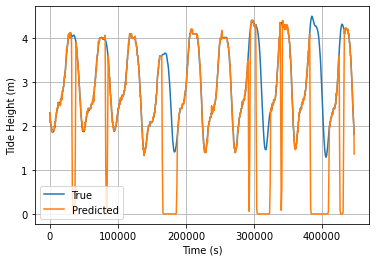
\includegraphics[width=8cm]{Figures/Graph 1.png}\label{fig:fig1}}
      \hfill
    \subfloat[With White Kernel (RMS error = 0.667)]{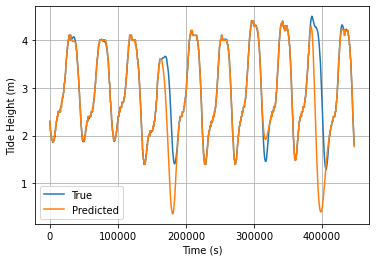
\includegraphics[width=8cm]{Figures/Graph 2.png}\label{fig:fig2}}
    \hfill
    \caption{Predicted values}
  \end{figure}
  
  \section{Exponential Sine Squared}
  \label{sec:ESS}
  The data set exhibits periodic behaviour, with a period of roughly 50000 seconds. Hence, we attempt to use a kernel which can model periodicity. 
  
  Figure \ref{fig:fig3} is similar to Figure \ref{fig:fig2} despite not including a White Kernel. However, the former retains the inaccurate predictions at the same points but has a lower RMS error. On the other hand, Figure \ref{fig:fig4} (RMS error of 0.192) gives the best predictions without the same errors present in Figures \ref{fig:fig2} and \ref{fig:fig3} (RMS error of 0.433). Again, including a White Kernel improved performance. These results seem to validate our assumptions that a periodic kernel would be a better model of the data.


  
  \begin{figure}[!htb]
      \centering
      \subfloat[Without White Kernel (RMS error = 0.433)]{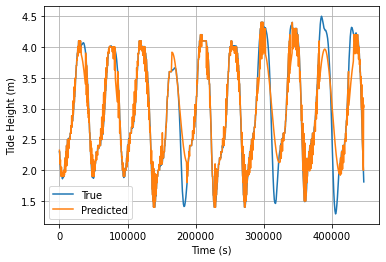
\includegraphics[width=8cm]{Figures/Graph 3.png}\label{fig:fig3}}
        \hfill
      \subfloat[With White Kernel (RMS error = 0.192)]{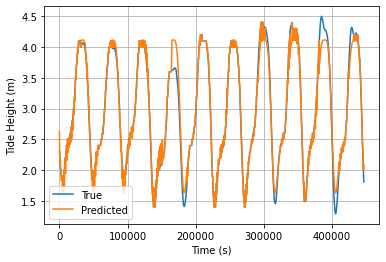
\includegraphics[width=8cm]{Figures/Graph 4.png}\label{fig:fig4}}
      \hfill
      \caption{Predicted values}
    \end{figure}
    
  

\end{document}

